% !TEX TS-program = knitr
\documentclass[handout]{beamer}\usepackage{graphicx, color}
%% maxwidth is the original width if it is less than linewidth
%% otherwise use linewidth (to make sure the graphics do not exceed the margin)
\makeatletter
\def\maxwidth{ %
  \ifdim\Gin@nat@width>\linewidth
    \linewidth
  \else
    \Gin@nat@width
  \fi
}
\makeatother

\IfFileExists{upquote.sty}{\usepackage{upquote}}{}
\definecolor{fgcolor}{rgb}{0.2, 0.2, 0.2}
\newcommand{\hlnumber}[1]{\textcolor[rgb]{0,0,0}{#1}}%
\newcommand{\hlfunctioncall}[1]{\textcolor[rgb]{0.501960784313725,0,0.329411764705882}{\textbf{#1}}}%
\newcommand{\hlstring}[1]{\textcolor[rgb]{0.6,0.6,1}{#1}}%
\newcommand{\hlkeyword}[1]{\textcolor[rgb]{0,0,0}{\textbf{#1}}}%
\newcommand{\hlargument}[1]{\textcolor[rgb]{0.690196078431373,0.250980392156863,0.0196078431372549}{#1}}%
\newcommand{\hlcomment}[1]{\textcolor[rgb]{0.180392156862745,0.6,0.341176470588235}{#1}}%
\newcommand{\hlroxygencomment}[1]{\textcolor[rgb]{0.43921568627451,0.47843137254902,0.701960784313725}{#1}}%
\newcommand{\hlformalargs}[1]{\textcolor[rgb]{0.690196078431373,0.250980392156863,0.0196078431372549}{#1}}%
\newcommand{\hleqformalargs}[1]{\textcolor[rgb]{0.690196078431373,0.250980392156863,0.0196078431372549}{#1}}%
\newcommand{\hlassignement}[1]{\textcolor[rgb]{0,0,0}{\textbf{#1}}}%
\newcommand{\hlpackage}[1]{\textcolor[rgb]{0.588235294117647,0.709803921568627,0.145098039215686}{#1}}%
\newcommand{\hlslot}[1]{\textit{#1}}%
\newcommand{\hlsymbol}[1]{\textcolor[rgb]{0,0,0}{#1}}%
\newcommand{\hlprompt}[1]{\textcolor[rgb]{0.2,0.2,0.2}{#1}}%

\usepackage{framed}
\makeatletter
\newenvironment{kframe}{%
 \def\at@end@of@kframe{}%
 \ifinner\ifhmode%
  \def\at@end@of@kframe{\end{minipage}}%
  \begin{minipage}{\columnwidth}%
 \fi\fi%
 \def\FrameCommand##1{\hskip\@totalleftmargin \hskip-\fboxsep
 \colorbox{shadecolor}{##1}\hskip-\fboxsep
     % There is no \\@totalrightmargin, so:
     \hskip-\linewidth \hskip-\@totalleftmargin \hskip\columnwidth}%
 \MakeFramed {\advance\hsize-\width
   \@totalleftmargin\z@ \linewidth\hsize
   \@setminipage}}%
 {\par\unskip\endMakeFramed%
 \at@end@of@kframe}
\makeatother

\definecolor{shadecolor}{rgb}{.97, .97, .97}
\definecolor{messagecolor}{rgb}{0, 0, 0}
\definecolor{warningcolor}{rgb}{1, 0, 1}
\definecolor{errorcolor}{rgb}{1, 0, 0}
\newenvironment{knitrout}{}{} % an empty environment to be redefined in TeX

\usepackage{alltt}
\newcommand{\answers}{1}

\usetheme{Marburg}
\setbeamertemplate{navigation symbols}{} 
\setbeamertemplate{footline}
{
  \leavevmode%
  \hbox{%
  \begin{beamercolorbox}[wd=.333333\paperwidth,ht=2.25ex,dp=1ex,center]{author in head/foot}%
    \usebeamerfont{author in head/foot}\copyright $\ $ \insertshortauthor%~~\beamer@ifempty{\insertshortinstitute}{}{(\insertshortinstitute)}
  \end{beamercolorbox}%
  \begin{beamercolorbox}[wd=.333333\paperwidth,ht=2.25ex,dp=1ex,center]{title in head/foot}%
    \usebeamerfont{title in head/foot} \insertinstitute
  \end{beamercolorbox}%
  \begin{beamercolorbox}[wd=.333333\paperwidth,ht=2.25ex,dp=1ex,right]{date in head/foot}%
    \usebeamerfont{date in head/foot}\insertshortdate{}\hspace*{2em}
    \insertframenumber{} / \inserttotalframenumber\hspace*{2ex} 
  \end{beamercolorbox}}%
  \vskip0pt%
}

\usepackage{amsmath}
\usepackage{caption}
\usepackage{color}
\usepackage{enumerate}
\usepackage{listings}
\usepackage{hyperref}
\usepackage{mathrsfs}
\usepackage{natbib}
\usepackage{url}

\providecommand{\all}{\ \forall \ }
\providecommand{\bs}{\backslash}
\providecommand{\e}{\varepsilon}
\providecommand{\E}{\ \exists \ }
\providecommand{\lm}[2]{\lim_{#1 \rightarrow #2}}
\providecommand{\m}[1]{\mathbb{#1}}
\providecommand{\nv}{{}^{-1}}
\providecommand{\ov}[1]{\overline{#1}}
\providecommand{\p}{\newpage}
\providecommand{\q}{$\quad$ \newline}
\providecommand{\rt}{\rightarrow}
\providecommand{\Rt}{\Rightarrow}
\providecommand{\vc}[1]{\boldsymbol{#1}}
\providecommand{\wh}[1]{\widehat{#1}}

\hypersetup{colorlinks,linkcolor=,urlcolor=blue}
\numberwithin{equation}{section}

\definecolor{dkgreen}{rgb}{0,0.6,0}
\definecolor{gray}{rgb}{0.5,0.5,0.5}
\definecolor{mauve}{rgb}{0.58,0,0.82}

\lstset{ 
  language=C,                % the language of the code
  basicstyle= \footnotesize,           % the size of the fonts that are used for the code
  numberstyle= \tiny \color{white},  % the style that is used for the line-numbers
  stepnumber=2,                   % the step between two line-numbers. 
  numbersep=5pt,                  % how far the line-numbers are from the code
  backgroundcolor=\color{white},      % choose the background color. You must add \usepackage{color}
  showspaces=false,               % show spaces adding particular underscores
  showstringspaces=false,         % underline spaces within strings
  showtabs=false,                 % show tabs within strings adding particular underscores
  frame=lrb,                   % adds a frame around the code
  rulecolor=\color{black},        % if not set, the frame-color may be changed on line-breaks within not-black text 
  tabsize=2,                      % sets default tabsize to 2 spaces
  captionpos=t,                   % sets the caption-position 
  breaklines=true,                % sets automatic line breaking
  breakatwhitespace=false,        % sets if automatic breaks should only happen at whitespace
  %title=\lstname,                   % show the filename of files included with \lstinputlisting;
  keywordstyle=\color{blue},          % keyword style
  commentstyle=\color{gray},       % comment style
  stringstyle=\color{dkgreen},         % string literal style
  escapeinside={\%*}{*)},            % if you want to add LaTeX within your code
  morekeywords={*, ...},               % if you want to add more keywords to the set
  xleftmargin=0.053in, % left horizontal offset of caption box
  xrightmargin=-.03in % right horizontal offset of caption box
}

%\DeclareCaptionFont{white}{\color{white}}
%\DeclareCaptionFormat{listing}{\parbox{\textwidth}{\colorbox{gray}{\parbox{\textwidth}{#1#2#3}}\vskip-0.05in}}
%\captionsetup[lstlisting]{format = listing, labelfont = white, textfont = white}
%For caption-free listings, comment out the 3 lines above and uncomment the 2 lines below.
 \captionsetup{labelformat = empty, labelsep = none}
 \lstset{frame = single}




\title{Inference for Multiple Regression}
\author{Will Landau}
\date{Apr 18, 2013}
\institute{Iowa State University}

\begin{document}

\begin{frame}
\titlepage
 \end{frame}
 
 \AtBeginSection[]
{
   \begin{frame}
       \frametitle{Outline}
       \tableofcontents[currentsection]
   \end{frame}
}

\section{Multiple Regression: a Review}

\begin{frame}
\frametitle{Multiple Regression} \small
\begin{itemize}
\item {\bf Multiple Regression}: regression on multiple variables:
\pause \begin{align*}
y_i \approx b_0 + b_1 x_{i, 1} + b_2 x_{i, 2} + b_3 x_{i,3} + \cdots + b_{p-1} x_{i, p- 1}
\end{align*}
\begin{itemize}
\pause \item The $p$ coefficients $b_0, b_1, \ldots, b_{p-1}$ are estimated by minimizing the loss function below using the least squares principle:
\end{itemize}
\pause \begin{align*}
S(b_0, b_1, \ldots, b_{p-1}) = \sum_{i = 1}^n (y_i -  b_0 + b_1 x_{i, 1} + \cdots + b_{p-1} x_{i,p- 1})^2
\end{align*}
\begin{itemize}
\pause \item In practice, we make a computer find the coefficients for us. This class uses JMP 10, a statistical software tool.
\end{itemize}
\end{itemize}
\end{frame}

\begin{frame}
\frametitle{Formalizing the multiple regression model}
\begin{itemize}
\item Now, we'll work with a formal multiple regression model:
\pause \begin{align*}
Y_i = \beta_0 + \beta_1 x_{1, i} + \beta_2 x_{2, i} + \cdots + \beta_{p-1} x_{p-1, i} + \e_i
\end{align*}
\pause \item Assume $\e_1, \e_2, \ldots, \e_n \sim$ iid $N(0,\sigma^2)$.
\end{itemize}
\begin{center}
\setkeys{Gin}{width=.8\textwidth} 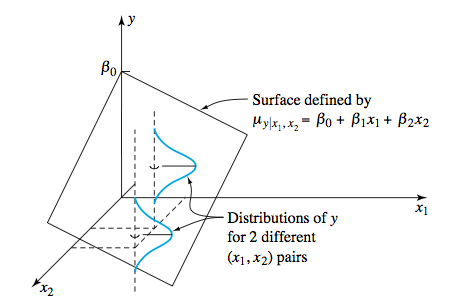
\includegraphics{../../fig/mulregpict.png}
\end{center}
\end{frame}


\section{Estimating $\sigma^2$}

\begin{frame}
\frametitle{Estimating $\sigma^2$}
\begin{itemize}
\item Now, the residuals are of the form:
\begin{align*}
\uncover<2->{e_i} &\uncover<2->{= y_i - \wh{y}_i} \\
&\uncover<3->{= y_i - (b_0 + b_1 x_{1,i} + \cdots + b_{p-1} x_{p-1,i})}
\end{align*}
\uncover<4->{\item We estimate the variance with the {\bf surface-fitting sample variance}, also called {\bf mean squared error (MSE)}:}
\begin{align*}
\uncover<5->{s^2_{SF} = \frac{1}{n-p} \sum e_i^2}
\end{align*}
\uncover<6->{\item The estimated standard deviation is $s_{SF} = \sqrt{s_{SF}^2}$.}
\uncover<7->{\item Note: the line fitting sample variance $s_{LF}^2$ is the special case of $s_{SF}^2$ for $p = 2$.}
\end{itemize}
\end{frame}

\begin{frame}
\frametitle{Example: stack loss}
\begin{enumerate}[1. ]
\item Consider a chemical plant that makes nitric acid from ammonia.
\uncover<2->{\item We want to predict stack loss ($y$, 10 times the \% ammonia that escapes from the absorption column) using:}
\begin{itemize}
\uncover<3->{\item $x_1$: air flow, the rate of operation of the plant}
\uncover<4->{\item $x_2$, inlet temperature of the cooling water}
\uncover<5->{\item $x_3$: (\% circulating acid - 50\% )$\times 10$}
\end{itemize}
\end{enumerate}
\end{frame}

\begin{frame}
\frametitle{Example: stack loss}
\setkeys{Gin}{width=1\textwidth} 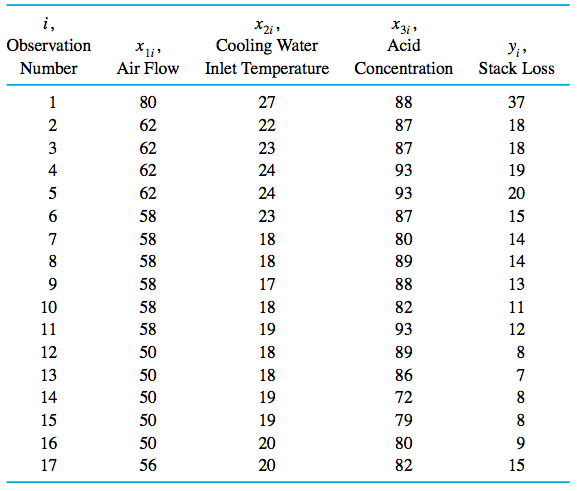
\includegraphics{../../fig/stack.png}
\end{frame}

\begin{frame}
\frametitle{Fitted surface: $\wh{y}_i = -37.65 + 0.797 x_{1, i} + 0.577 x_{2, i} - 0.067 x_{3, i}$}
\begin{center}
\setkeys{Gin}{width=.7\textwidth} 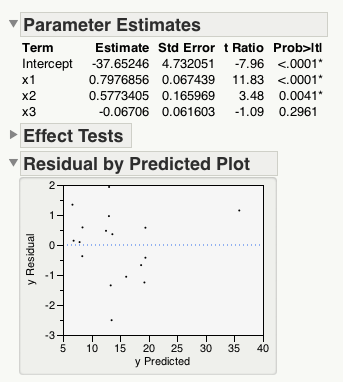
\includegraphics{../../fig/stackoutput.png}
\end{center}
\end{frame}


\begin{frame}
\frametitle{Example: stack loss}
\begin{center}
\setkeys{Gin}{width=.7\textwidth} 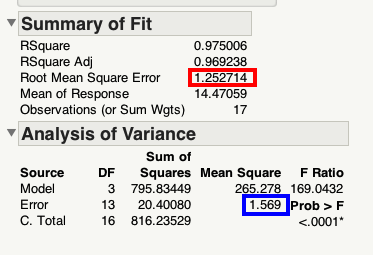
\includegraphics{../../fig/stackmse.png}
\begin{itemize}
\item $s_{SF}^2 = 1.569$ (``Mean Square Error", blue)
\uncover<2->{\item $s_{SF} = \sqrt{1.569} = 1.25$, also under ``Root Mean Square Error" (red).}
\end{itemize}
\end{center}
\end{frame}

\section{Standardized Residuals}

\begin{frame}
\frametitle{Standardized residuals}
\begin{itemize}
\item As with simple linear regression, Var($e_i$) is not constant even though Var($\e_i$) = $\sigma^2$. 
\uncover<2->{\item There are some constants $a_1, a_2, \ldots, a_n$ such that:}
\begin{align*}
\uncover<3->{Var(e_i) = a_i \sigma^2}
\end{align*}
\uncover<4->{\item Hence, we compute the standardized residuals as:}
\begin{align*}
\uncover<5->{e_i^* = \frac{e_i}{s_{SF} \sqrt{a_i}}}
\end{align*}
\uncover<6->{\item In practice, $a_1, \ldots, a_n$ are hard to compute. We'll make JMP do all the hard work.}
\end{itemize}
\end{frame}

\begin{frame}
\frametitle{Example: stack loss}
\setkeys{Gin}{width=1\textwidth} 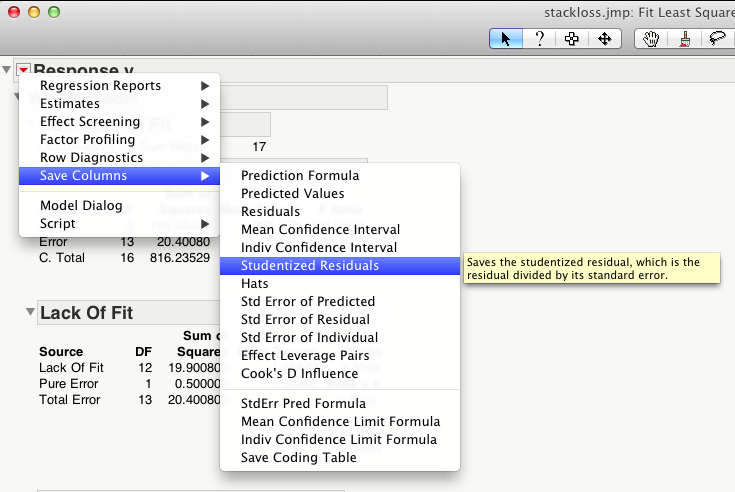
\includegraphics{../../fig/stackstd1.png}
\end{frame}

\begin{frame}
\frametitle{Example: stack loss}
\setkeys{Gin}{width=1\textwidth} 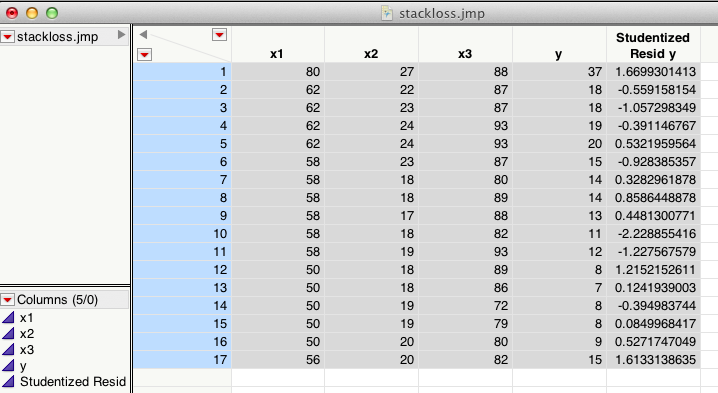
\includegraphics{../../fig/stackstd2.png}
\end{frame}


\begin{frame}
\frametitle{Example: stack loss}
\setkeys{Gin}{width=1\textwidth} 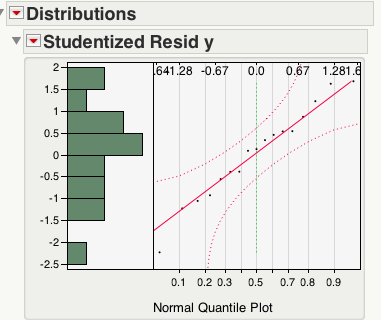
\includegraphics{../../fig/stackstd3.png}
\end{frame}




\section{Inference for $\beta_0, \beta_1, \ldots, \beta_{p-1}$}

\begin{frame}
\frametitle{Inference for $\beta_0, \beta_1, \ldots, \beta_{p-1}$}
\begin{itemize}
\item Our formal model is:
\begin{align*}
Y_i = \beta_0 + \beta_1 x_{1, i} + \beta_2 x_{2, i} + \cdots + \beta_{p-1} x_{p-1, i} + \e_i
\end{align*}
\pause \item Our estimated model is:
\begin{align*}
\wh{y}_i = b_0 +b_1 x_{1, i} +b_2 x_{2, i} + \cdots + b_{p-1} x_{p-1, i} 
\end{align*}
\pause \item How close are the estimates to their true values?
\end{itemize}
\end{frame}

\begin{frame}
\frametitle{Inference for $\beta_0, \beta_1, \ldots, \beta_{p}$}
\begin{itemize}
\item Under our model assumptions:
\begin{align*}
b_l \sim N(\beta_l, d_l \sigma^2)
\end{align*}
for some positive constant $d_l$, $l = 0, 1, 2, \ldots, p-1$.
\pause \item That means:
\begin{align*}
\frac{b_l - \beta_l}{s_{SF} \sqrt{d_l}} = \frac{b_l - \beta_l}{\wh{SD}(b_l)} \sim t_{n - p}
\end{align*}
\pause \item A test statistic for testing $H_0: b_l = \#$ is:
\begin{align*}
K = \frac{b_l - \#}{s_{SF} \sqrt{d_l}} = \frac{b_l - \#}{\wh{SD}(b_l)} \sim t_{n-p}
\end{align*}
\pause \item A 2-sided $1 - \alpha$ confidence interval for $\beta_l$ is:
\begin{align*}
\uncover<5->{b_l \pm t_{n - p, \ 1 - \alpha/2} \cdot s_{SF} \sqrt{d_l}}
\intertext{\uncover<6->{i.e.,}}
\uncover<6->{b_l \pm t_{n - p, \ 1 - \alpha/2} \cdot \wh{SD}(d_l)}
\end{align*} 
\end{itemize}
\end{frame}







\begin{frame}
\frametitle{Your turn} \scriptsize
\begin{itemize}
\item $n = 17$
\item $x_1$: air flow, the rate of operation of the plant
\pause \item $x_2$, inlet temperature of the cooling water
\pause \item $x_3$: (\% circulating acid - 50\% )$\times 10$
\end{itemize}
\begin{center}
\setkeys{Gin}{width=.7\textwidth} 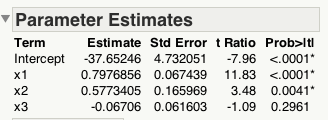
\includegraphics{../../fig/stackparams.png}
\end{center}
\begin{enumerate}[1. ]
\pause \item Test $H_0: \beta_1 = 1$ vs. $H_a: \beta_1 < 1$ using $\alpha = 0.1$. 
\pause \item Test $H_0: \beta_3 = 0$ vs. $H_a: \beta_3 \ne 0$ by hand ($\alpha = 0.05$), and compare your t statistic to the one in the output table.
\pause \item Construct and interpret a 2-sided 99\% confidence interval for $\beta_3$. 
\pause \item Construct and interpret a 1-sided lower 90\% confidence interval for $\beta_2$
\end{enumerate}
\end{frame}

\begin{frame}<handout:\answers>
\frametitle{Answers: 1}
\begin{enumerate}[1. ]
\item $H_0: \beta_1 = 1$, $H_a: \beta_1 < 1$
\pause \item $\alpha = 0.1$
\pause \item I use the test statistic:
\pause \begin{align*}
K = \frac{b_1 - 1}{\wh{SD}(b_1)}
\end{align*}
\begin{itemize}
\pause \item I assume:
\begin{itemize}
\pause \item $H_0$ is true.
\pause \item The model $Y_i = \beta_0 + \beta_1 x_{1, i} + \beta_1 x_{2, i} + \beta_1 x_{3, i} + \e_i$, with $\e_1, \ldots, \e_{17} \sim N(0, \sigma^2)$ is correct.
\end{itemize}
\pause \item Under the assumptions, $K \sim t_{n - p} = t_{17 - 4} = t_{13}$.
\pause \item I will reject $H_0$ if $K< -t_{13, 1 - \alpha} = t_{13, 0.9} = 1.35$.
\end{itemize}
\end{enumerate}
\end{frame}


\begin{frame}<handout:\answers>
\frametitle{Answers: 1} \small
\begin{enumerate}
\setcounter{enumi}{3}
\item The moment of truth:
\pause \begin{align*}
K &= \frac{0.7977 - 1}{0.06744} = -3.00 \\
\end{align*}
\pause \item With $K = -3 <  -1.35 = -t_{13, 0.9}$, we reject $H_0$ and conclude $H_a$.
\pause \item There is enough evidence to conclude that the true slope on airflow is less than 1 unit stack loss / unit airflow. With each unit increase in airflow and all the other covariates held constant, we expect stack loss to increase by less than one unit.
\end{enumerate}
\end{frame}





\begin{frame}<handout:\answers>
\frametitle{Answers: 2}
\begin{enumerate}[1. ]
\item $H_0: \beta_3 = 0$, $H_a: \beta_3 \ne 0$
\pause \item $\alpha = 0.05$
\pause \item I use the test statistic:
\pause \begin{align*}
K = \frac{b_3 - 0}{\wh{SD}(b_3)}
\end{align*}
\begin{itemize}
\pause \item I assume:
\begin{itemize}
\pause \item $H_0$ is true.
\pause \item The model $Y_i = \beta_0 + \beta_1 x_{1, i} + \beta_1 x_{2, i} + \beta_1 x_{3, i} + \e_i$, with $\e_1, \ldots, \e_{17} \sim N(0, \sigma^2)$ is correct.
\end{itemize}
\pause \item Under the assumptions, $K \sim t_{n - p} = t_{17 - 4} = t_{13}$.
\pause \item I will reject $H_0$ if $|K| > | t_{13, 1 - \alpha/2} |= t_{13, 0.975} = 2.16$.
\end{itemize}
\end{enumerate}
\end{frame}


\begin{frame}<handout:\answers>
\frametitle{Answers: 2} \small
\begin{enumerate}
\setcounter{enumi}{3}
\item The moment of truth:
\begin{align*}
\uncover<2->{K} & \uncover<2->{= \frac{-0.06706 - 0}{0.0616} = -1.089 \quad \text{\scriptsize (agrees with the ``t Ratio")}} \\
\end{align*}
\uncover<3->{\item With $ |K| = 1.089 < 2.16$, we fail to reject $H_0$.}
\uncover<4->{\item There is not enough evidence to conclude that the true slope on circulating acid (shifted and scaled) is nonzero. With each unit increase acid and all the other covariates held constant, there is no evidence that the stack loss should change.}
\end{enumerate}
\end{frame}


\begin{frame}<handout:\answers>
\frametitle{Answers: 3} \small
\begin{itemize}
\item For a confidence level of $99\%$, $\alpha = 0.01$ and so $t_{n - p, 1 - \alpha/2} = t_{13, 0.995} = 3.012$.
\end{itemize}
\begin{align*}
&\uncover<2->{(b_3 - t_{n - p, 1 - \alpha/2} \cdot \wh{SD}(b_3), \ b_3 + t_{n - p, 1 - \alpha/2}\cdot \wh{SD}(b_3))} \\
&\uncover<3->{=  (-0.06706 - 3.012 \cdot 0.0616, \ -0.06706 + 3.012 \cdot 0.0616)} \\
&\uncover<4->{= (-0.2525, \ 0.1185)}
\end{align*}
\begin{itemize}
\uncover<5->{\item We're 99\% confident that, for every unit increase in acid with all other covariates held constant, stack loss increases by anywhere from -0.2525 units to 0.1185 units.}
\end{itemize}
\end{frame}


\begin{frame}<handout:\answers>
\frametitle{Answers: 4} \small
\begin{itemize}
\item For a confidence level of $90\%$, $\alpha = 0.1$ and so $t_{n - p, 1 - \alpha/2} = t_{13, 0.95} =1.77$.
\end{itemize}
\begin{align*}
&\uncover<2->{(b_2 - t_{n - p, 1 - \alpha/2} \cdot \wh{SD}(b_2), \ b_2 + t_{n - p, 1 - \alpha/2}\cdot \wh{SD}(b_2))} \\
&\uncover<3->{=  (0.5573 - 1.77 \cdot 0.166, \ 0.5573 +1.77 \cdot 0.166)} \\
&\uncover<4->{= (0.26348, \ 0.8511)}
\end{align*}
\begin{itemize}
\uncover<5->{\item We're 90\% confident that, for every 1-degree increase in temperature with all other covariates held constant, stack loss increases by anywhere from 0.26348 units to 0.8511 units.}
\end{itemize}
\end{frame}





\section{Inference for Mean Responses}

\subsection{Individual mean responses}


\begin{frame}
\frametitle{Individual mean responses} \scriptsize
\begin{itemize}
\item We want to estimate the mean response at the set of covariate values, ($x_1, x_2, \ldots, x_{p-1}$)
\uncover<2->{\item Under the model assumptions, the estimated mean response, $\wh{\mu}_{y \mid \vc{x}}$, at $\vc{x} = $ ($x_1, x_2, \ldots, x_{p-1}$) is normally distributed with:}
\begin{align*}
\uncover<3->{E(\wh{\mu}_{y \mid \vc{x}})} &\uncover<3->{= \mu_{y \mid \vc{x}} = \beta_0 + \beta_1 x_1 + \cdots + \beta_{p-1} x_{p-1}} \\
\uncover<4->{Var(\wh{\mu}_{y \mid \vc{x}})} & \uncover<4->{= \sigma^2 A^2}
\end{align*}
\uncover<4->{for some constant $A$.}
\uncover<5->{\item Under the model assumptions:}
\begin{align*}
\uncover<6->{Z = \frac{\wh{\mu}_{y \mid \vc{x}} - \mu_{y \mid \vc{x}}}{\sigma A} \sim N(0,1) \quad T = \frac{\wh{\mu}_{y \mid \vc{x}} - \mu_{y \mid \vc{x}}}{s_{SF} A}  \sim t_{n - p}}
\end{align*}
\uncover<7->{\item A test statistic for testing $H_0:  \mu_{y \mid \vc{x}} = \#$ is:}
\begin{align*}
\uncover<8->{ \frac{{\wh{\mu}_{y \mid \vc{x}} - \#}}{s_{SF} A}}
\end{align*}
\uncover<8->{which has a $t_{n - p}$ distribution under $H_0$.}
\uncover<9->{\item A 2-sided, $1 - \alpha$ confidence interval for $\mu_{y \mid \vc{x}}$ in compact form is $\wh{\mu}_{y \mid \vc{x}} \pm t_{n - p, 1 - \alpha/2} \cdot s_{SF} \cdot A$.}
\uncover<10->{\item Note: $s_{SF} A$ = $\wh{SD}(\wh{\mu}_{y \mid \vc{x}})$, which you can get directly from JMP output.}
\end{itemize}
\end{frame}

\begin{frame}
\frametitle{Example: stack loss}
\begin{itemize}
\item  I will use JMP to compute a 2-sided 95\% confidence interval around the mean response at point 3: $x_1 = 62, x_2 = 23, x_3 = 87, y = 18$. 
\end{itemize}
\end{frame}

\begin{frame}
\frametitle{Example: stack loss}
\setkeys{Gin}{width=1\textwidth} 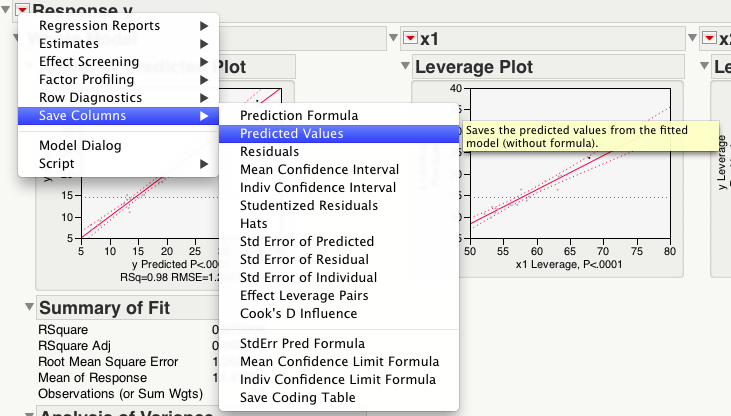
\includegraphics{../../fig/mmc1.png}
\end{frame}

\begin{frame}
\frametitle{Example: stack loss}
\setkeys{Gin}{width=1\textwidth} 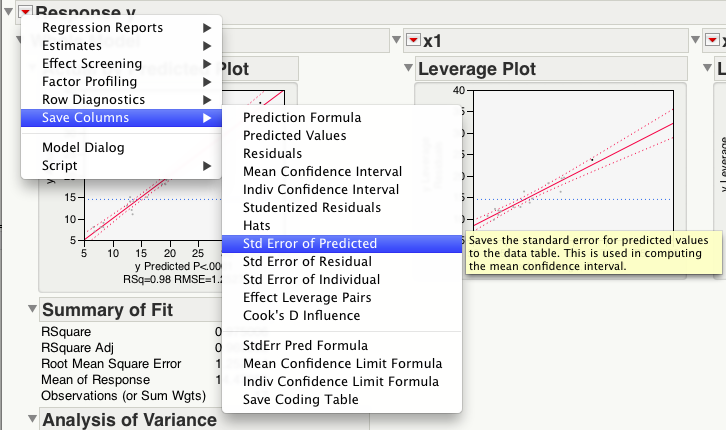
\includegraphics{../../fig/mmc2.png}
\end{frame}

\begin{frame}
\frametitle{Example: stack loss}
\setkeys{Gin}{width=1\textwidth} 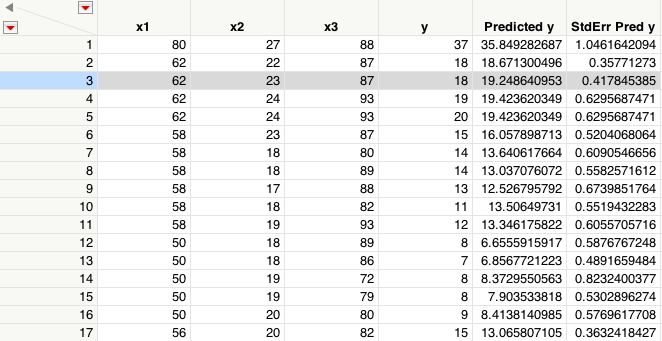
\includegraphics{../../fig/mmc3.png}
\end{frame}


\begin{frame}
\frametitle{Example: stack loss}
\begin{itemize}
\item With $t_{n - p, 1 - \alpha/2} = t_{13, 0.975} = 2.16$ the confidence interval is:
\end{itemize}
\begin{align*}
&\uncover<2->{(\wh{\mu}_{y \mid \vc{x}} - 2.16 \cdot \wh{SD}(\wh{\mu}_{y \mid \vc{x}}), \ \wh{\mu}_{y \mid \vc{x}} + 2.16 \cdot \wh{SD}(\wh{\mu}_{y \mid \vc{x}}))} \\
&\uncover<3->{= (19.249 - 2.16 \cdot 0.419, \ 19.249 + 2.16 \cdot 0.419)} \\
&\uncover<4->{= (10.199, \ 28.299)}
\end{align*}
\begin{itemize}
\uncover<5->{\item We're 95\% confident that when the air flow is 62, the temperature is 23 degrees, and the adjusted percentage of circulating acid is 87, the true mean stack loss is anywhere between 10.199 and 28.299 units.}
\end{itemize}
\end{frame}



\subsection{Multiple mean responses}

\begin{frame}
\frametitle{Multiple mean responses}
\begin{itemize}
\item The multiple $1 - \alpha$ confidence interval formula for $\mu_{y \mid x_1, \ldots, x_{p-1}}$ is:
\begin{align*}
\wh{\mu}_{y \mid \vc{x}} \pm \sqrt{p \cdot F_{p, \ n - p, \ 1 - \alpha }} \cdot s_{SF} \cdot A
\end{align*}
\pause \item Since there's no simple formula for $A$, we'll make JMP do all the work for us.
\pause \item First, we'll need to write $\wh{SD}(\wh{\mu}_{y \mid \vc{x}}) = s_{SF} \cdot A$ and write the interval as:
\begin{align*}
\wh{\mu}_{y \mid \vc{x}} \pm \sqrt{p \cdot F_{p, \ n - p, \ 1 - \alpha}} \cdot \wh{SD}(\wh{\mu}_{y \mid \vc{x}})
\end{align*}
\end{itemize}
\end{frame}


\begin{frame}
\frametitle{Example: stack loss}
\begin{itemize}
\item With $p$ parameters and 95\% confidence intervals, $F_{p, \ n - p, \ 1 - \alpha} = F_{4, 13, 0.95} = 3.18$.
\uncover<2->{\item The multiple confidence interval becomes:}
\begin{align*}
\uncover<3->{\wh{\mu}_{y \mid \vc{x}} \pm \sqrt{4 \cdot 3.18} \cdot \wh{SD}(\wh{\mu}_{y \mid \vc{x}})} \\
\intertext{\uncover<4->{i.e.,}}
\uncover<4->{\wh{\mu}_{y \mid \vc{x}} \pm 3.57 \cdot \wh{SD} (\wh{\mu}_{y \mid \vc{x}})}
\end{align*}
\uncover<5->{\item $\wh{\mu}_{y \mid \vc{x}}$ and $\wh{SD}(\wh{\mu}_{y \mid \vc{x}})$ vary from point to point.}
\end{itemize}
\end{frame}

\begin{frame}
\frametitle{Example: stack loss}
\setkeys{Gin}{width=.8\textwidth} 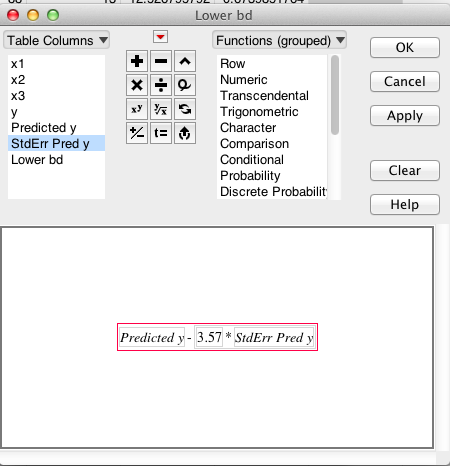
\includegraphics{../../fig/msl1.png}
\end{frame}

\begin{frame}
\frametitle{Example: stack loss}
\setkeys{Gin}{width=.9\textwidth} 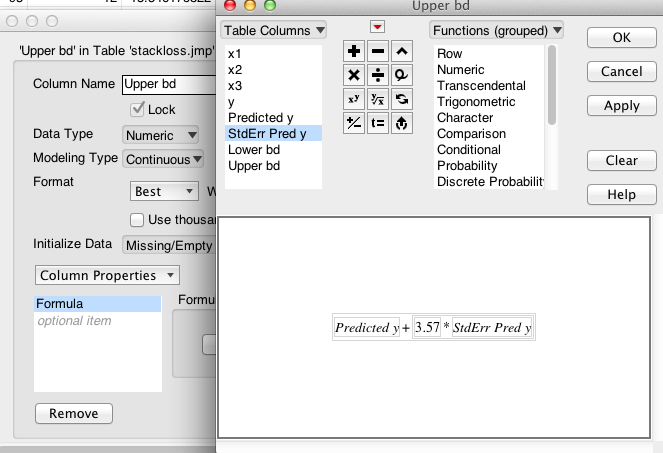
\includegraphics{../../fig/msl2.png}
\end{frame}

\begin{frame}
\frametitle{Example: stack loss}
\begin{itemize}
\item The columns, ``Lower bd" and ``Upper bd", give the endpoints for the confidence intervals.
\end{itemize}
\setkeys{Gin}{width=1\textwidth} 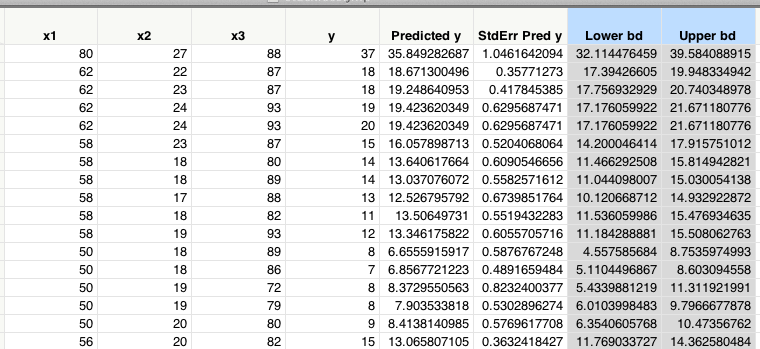
\includegraphics{../../fig/msl3.png}
\end{frame}



\end{document}
